\documentclass[letterpaper,12pt]{article}

\usepackage[vmargin=1cm, hmargin=1cm]{geometry}
\usepackage{fourier}
\usepackage{paralist}
\usepackage{amsmath}
\usepackage{amssymb}
\usepackage{graphicx}
\usepackage{booktabs}
\usepackage{tikz}
\usetikzlibrary{automata,arrows}
\begin{document}
\pagestyle{empty}
     \begin{center}
    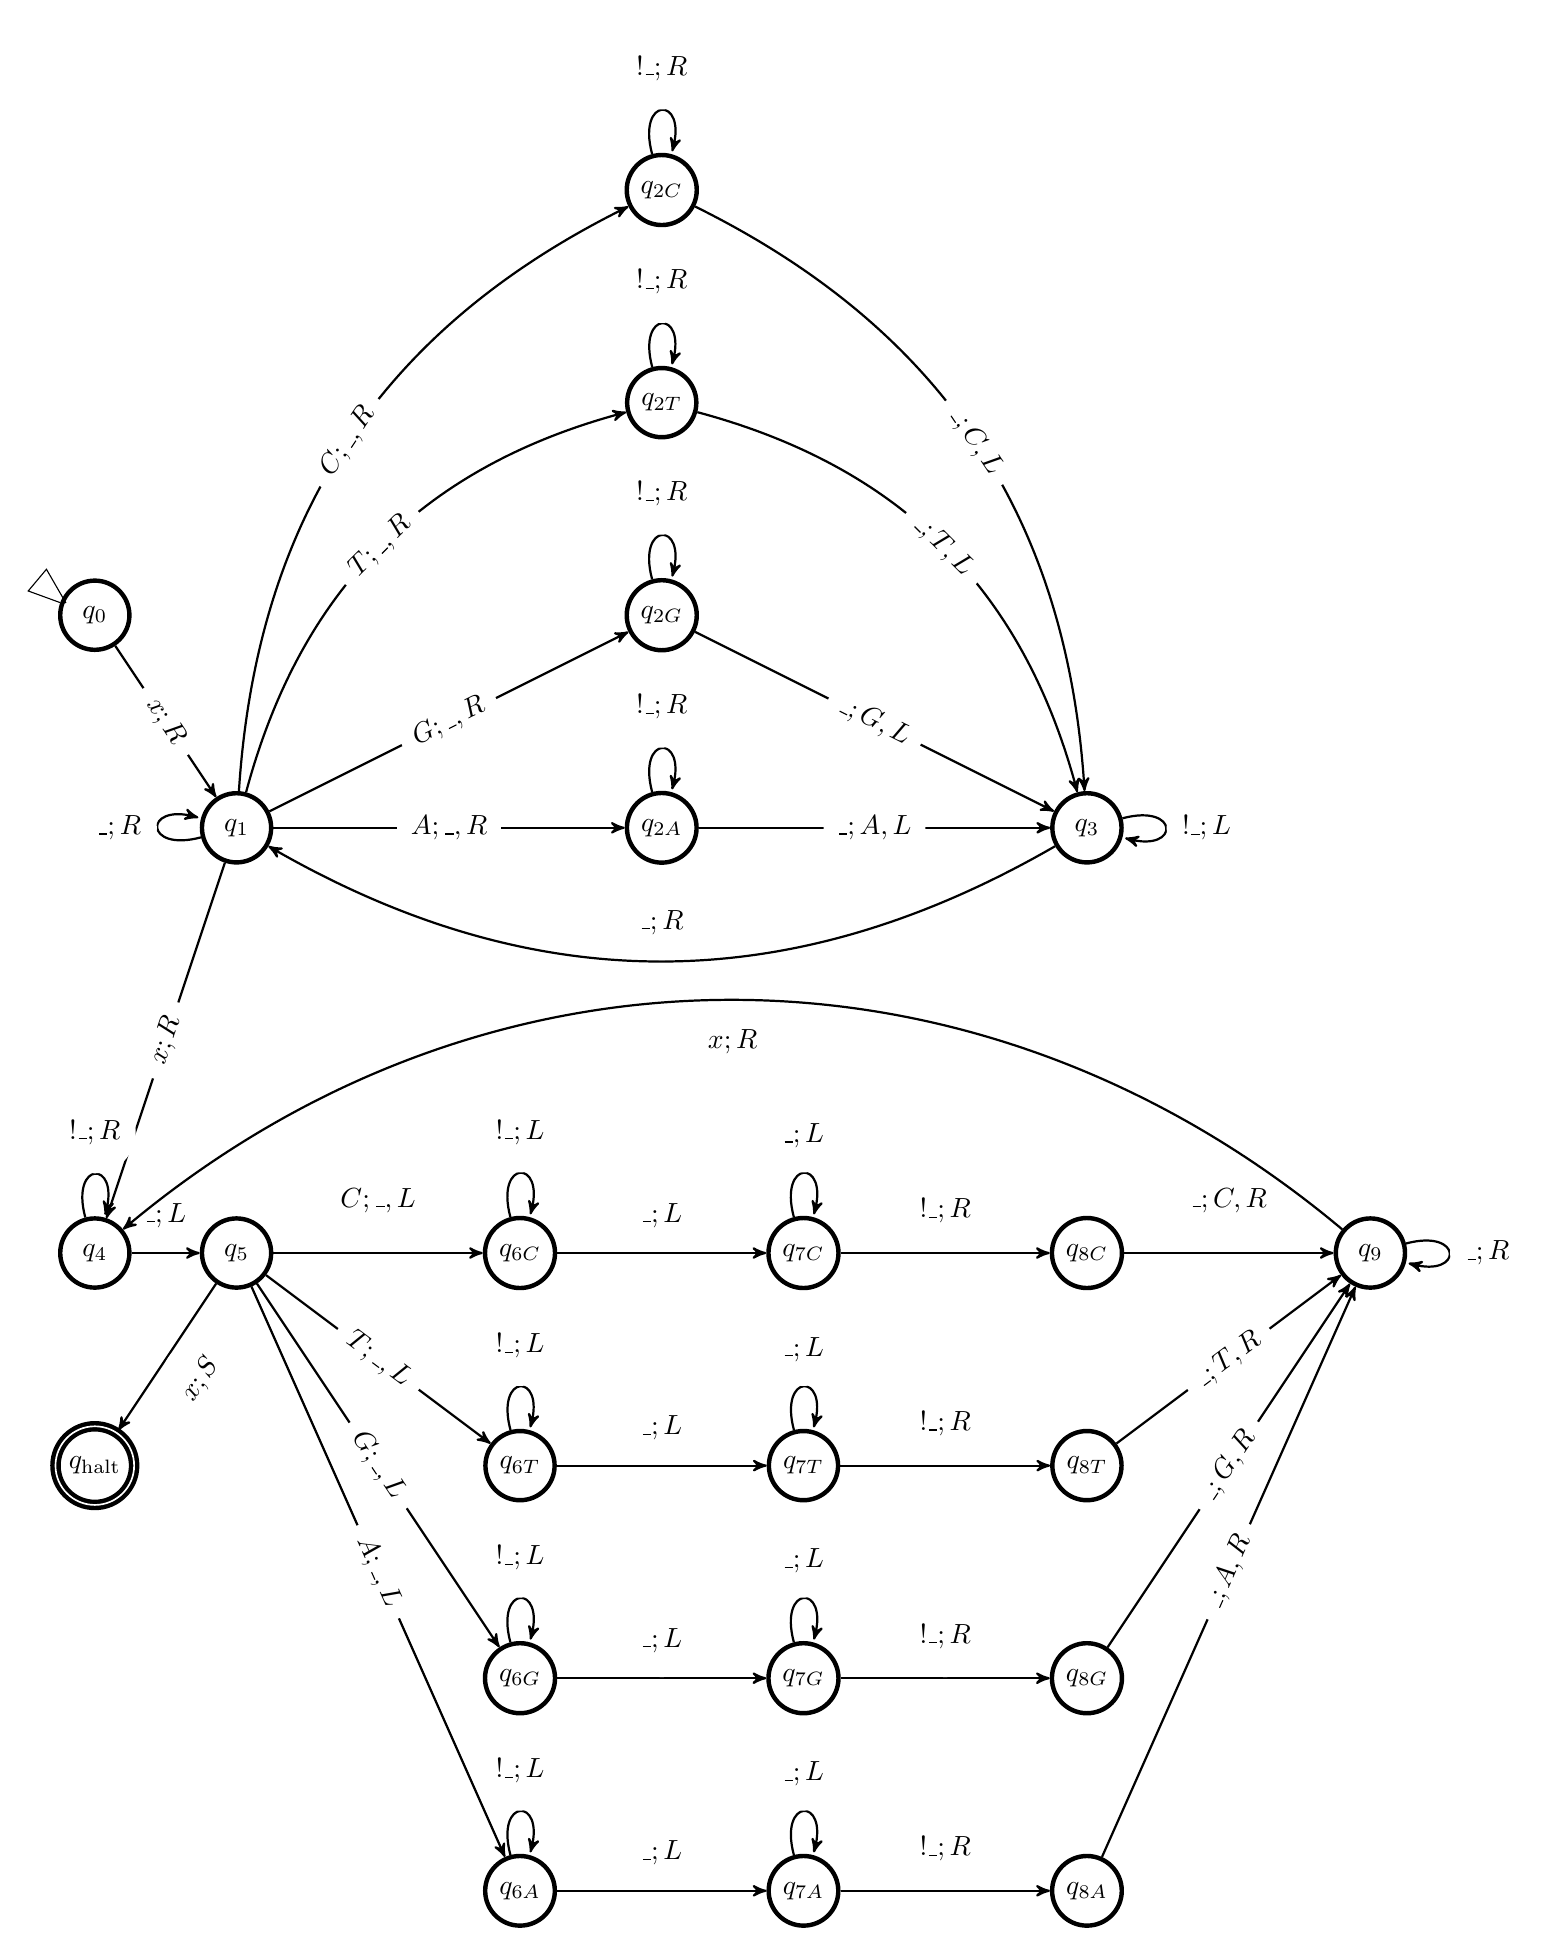
\begin{tikzpicture}[scale=0.9]
    \begin{scope}[every node/.style={circle,ultra thick,draw}]
        \node[state] (q0) at (0,7) {$q_0$};
        \node[state] (q1) at (2,4) {$q_1$};
        \node[state] (q2C) at (8,13) {$q_{2C}$};
        \node[state] (q2T) at (8,10) {$q_{2T}$};
        \node[state] (q2G) at (8,7) {$q_{2G}$};
        \node[state] (q2A) at (8,4) {$q_{2A}$};
        \node[state] (q3) at (14,4)  {$q_3$};
        \node[state] (q4) at (0,-2) {$q_4$};
        \node[state] (q5) at (2,-2) {$q_5$};
        \node[state] (q6C) at (6,-2) {$q_{6C}$};
        \node[state] (q7C) at (10,-2) {$q_{7C}$};
        \node[state] (q8C) at (14,-2) {$q_{8C}$};
        \node[state] (q6T) at (6,-5) {$q_{6T}$};
        \node[state] (q7T) at (10,-5) {$q_{7T}$};
        \node[state] (q8T) at (14,-5) {$q_{8T}$};
        \node[state] (q6G) at (6,-8) {$q_{6G}$};
        \node[state] (q7G) at (10,-8) {$q_{7G}$};
        \node[state] (q8G) at (14,-8) {$q_{8G}$};
        \node[state] (q6A) at (6,-11) {$q_{6A}$};
        \node[state] (q7A) at (10,-11) {$q_{7A}$};
        \node[state] (q8A) at (14,-11) {$q_{8A}$};
        \node[state] (q9) at (18,-2) {$q_{9}$};
        \node[state, accepting] (qH) at (0,-5) {$q_{\textrm{halt}}$};
    \end{scope}

    \begin{scope}[->,>=stealth',
                  every node/.style={fill=white, circle},
                  every edge/.style={draw=black, thick}]
        \path [->] (q0) edge[sloped] node {$x;R$} (q1);
        \path [->] (q1) edge[loop left] node {$\_;R$} (q1);
        \path [->] (q1) edge[bend left, sloped] node {$C;\_,R$} (q2C);
        \path [->] (q1) edge[bend left, sloped] node {$T;\_,R$} (q2T);
        \path [->] (q1) edge[sloped] node {$G;\_,R$} (q2G);
        \path [->] (q1) edge[sloped] node {$A;\_,R$} (q2A);
        \path [->] (q2C) edge[loop above] node {$!\_;R$} (q2C);
        \path [->] (q2T) edge[loop above] node {$!\_;R$} (q2T);
        \path [->] (q2G) edge[loop above] node {$!\_;R$} (q2G);
        \path [->] (q2A) edge[loop above] node {$!\_;R$} (q2A);
        \path [->] (q2C) edge[bend left, sloped] node {$\_;C,L$} (q3);
        \path [->] (q2T) edge[bend left, sloped] node {$\_;T,L$} (q3);
        \path [->] (q2G) edge[sloped] node {$\_;G,L$} (q3);
        \path [->] (q2A) edge[sloped] node {$\_;A,L$} (q3);
        \path [->] (q3) edge[loop right] node {$!\_;L$} (q3);
        \path [->] (q3) edge[bend left, above] node {$\_;R$} (q1);
        \path [->] (q1) edge[sloped] node {$x;R$} (q4);
        \path [->] (q4) edge[loop above] node {$!\_;R$} (q4);
        \path [->] (q4) edge[above] node {$\_;L$} (q5);
        \path [->] (q5) edge[above] node {$C;\_,L$} (q6C);
        \path [->] (q6C) edge[loop above] node {$!\_;L$} (q6C);
        \path [->] (q6C) edge[above] node {$\_;L$} (q7C);
        \path [->] (q7C) edge[loop above] node {$\_;L$} (q7C);
        \path [->] (q7C) edge[above] node {$!\_;R$} (q8C);
        \path [->] (q8C) edge[above] node {$\_;C,R$} (q9);
        \path [->] (q5) edge[sloped] node {$G;\_,L$} (q6G);
        \path [->] (q6G) edge[loop above] node {$!\_;L$} (q6G);
        \path [->] (q6G) edge[above] node {$\_;L$} (q7G);
        \path [->] (q7G) edge[loop above] node {$\_;L$} (q7G);
        \path [->] (q7G) edge[above] node {$!\_;R$} (q8G);
        \path [->] (q8G) edge[sloped] node {$\_;G,R$} (q9);
        \path [->] (q5) edge[sloped] node {$A;\_,L$} (q6A);
        \path [->] (q6A) edge[loop above] node {$!\_;L$} (q6A);
        \path [->] (q6A) edge[above] node {$\_;L$} (q7A);
        \path [->] (q7A) edge[loop above] node {$\_;L$} (q7A);
        \path [->] (q7A) edge[above] node {$!\_;R$} (q8A);
        \path [->] (q8A) edge[sloped] node {$\_;A,R$} (q9);
        \path [->] (q5) edge[sloped] node {$T;\_,L$} (q6T);
        \path [->] (q6T) edge[loop above] node {$!\_;L$} (q6T);
        \path [->] (q6T) edge[above] node {$\_;L$} (q7T);
        \path [->] (q7T) edge[loop above] node {$\_;L$} (q7T);
        \path [->] (q7T) edge[above] node {$!\_;R$} (q8T);
        \path [->] (q8T) edge[sloped] node {$\_;T,R$} (q9);
        \path [->] (q9) edge[loop right] node {$\_;R$} (q9);
        \path [->] (q9) edge[bend right=40, below] node {$x;R$} (q4);
        \path [->] (q5) edge[sloped, below] node {$x;S$} (qH);
    \end{scope}
    \draw (q0) -- ++(160:1) -- ++(50:0.4) -- ++(-60:0.55);
    \end{tikzpicture}
    \end{center}
\end{document}
